\documentclass[12pt]{article}
\usepackage{amsmath}
%\usepackage{fullpage}
\usepackage[top=1in, bottom=1in, left=0.8in, right=1in]{geometry}
\usepackage{multicol}
\usepackage{wrapfig}
\usepackage{graphicx}
\usepackage{float}
\usepackage{listings}
\usepackage{enumerate}
\lstset{language=Java,
basicstyle={\small\ttfamily},
columns=flexible,
belowskip=0mm}

\setlength{\columnsep}{0.1pc}

\title{ME573 Homework Set \# 5}
\author{Alexander Swenson -- \texttt{aaswenson@wisc.edu}}
\date{\today}
\begin{document}

  \maketitle

  \vspace{-0.3in}
  \noindent
  \rule{\linewidth}{0.4pt}

  \noindent
  
%%%%%%%%%%%%%%%%%%%%%%%%%%%%%%%%%%%%%%%%%%%%%%%%%%%%%%%%%%%%%%%%%%%%%%%%%%%%%%%%
% Problems 1

\section{Problem 1}

\noindent This problem solved the 1D heat diffusion equation using the forward in time, central in space method (FTCS). The scheme is as follows

\begin{equation}
\frac{f_i^{n+1} - f_i^n}{\Delta t}  = K \left(\frac{f_{i-1}^{n} - 2f_i^{n} + f_{i+1}^{n}}{\Delta x^2}\right) 
\label{eqn:ftcs_scheme}
\end{equation}

\noindent With initial conditions:

\begin{align*}
	f(x,0) = \begin{cases}
	U_o = const = 2 & \text{if} |x| < 1\\
	0 & \text{if} |x| > 1 
	\end{cases}
\end{align*}

\noindent The analytical solution is:

\begin{equation}
	f(x,t) = \frac{U_o}{2} \left[erf\left(\frac{(1-x)}{2\sqrt{kt}}\right) - erf\left(-\frac{(x+1)}{2\sqrt{kt}}\right)\right]
\end{equation}

\noindent The scheme was implemented with k = 1e-3, $\Delta t$ = 0.01, for various step sizes $\Delta x$ = [0.5, 0.25, 0.05], on the range [-3,3]. The results of the three grid refinements compared to the analytical solution are shown in Figure \ref{fig:problem1}.

\begin{figure}[H]
	\centering
	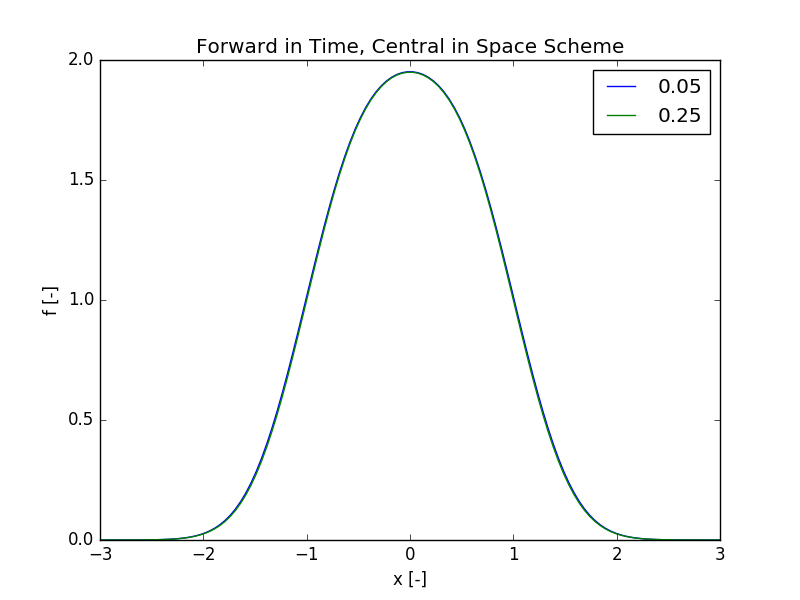
\includegraphics[height=3.75in]{problem1.png}
	\label{fig:problem1}
\end{figure}


%%%%%%%%%%%%%%%%%%%%%%%%%%%%%%%%%%%%%%%%%%%%%%%%%%%%%%%%%%%%%%%%%%%%%%%%%%%%%%%%


%%%%%%%%%%%%%%%%%%%%%%%%%%%%%%%%%%%%%%%%%%%%%%%%%%%%%%%%%%%%%%%%%%%%%%%%%%%%%%%%
% Problems:

\section{Problem 2}

\noindent In this problem, the heat diffusion equation was solved using both the forward in time, central in space method and the backward in time, central in space method (BTCS). The same initial conditions and constants from Problem 1 were used. The two schemes were compared to each other and the exact analytical solution. The comparison was made with a $\Delta x$ = 0.05 and two $\Delta t$ values (1, 2). Figure \ref{fig:problem2a} shows the results from a time step of 1.

\begin{figure}[H]
	\centering
	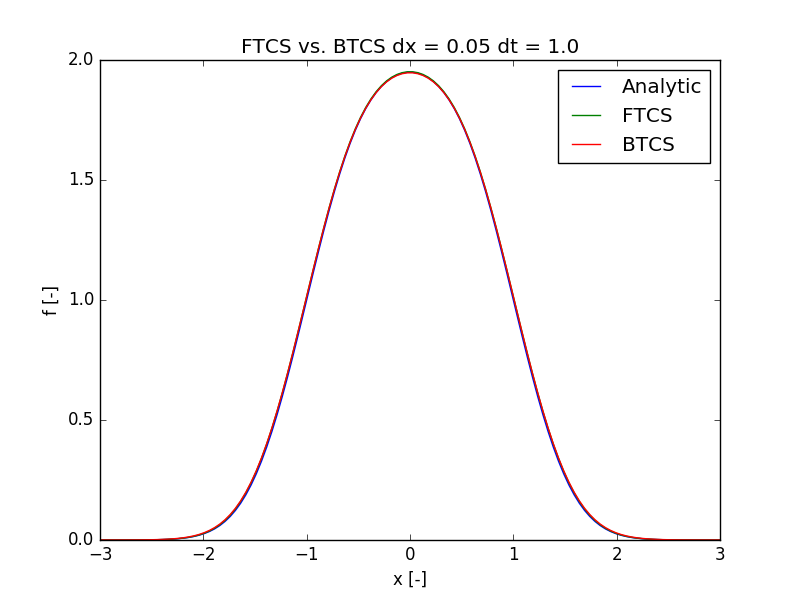
\includegraphics[height=3.75in]{problem2a.png}
	\label{fig:problem2a}
\end{figure}

Both the FTCS and BTCS are in good agreement with exact solution. Next, the same numerical schemes were compared using a time step of 2. Figure \ref{fig:problem2b} shows the results of this comparison.

\begin{figure}[H]
	\centering
	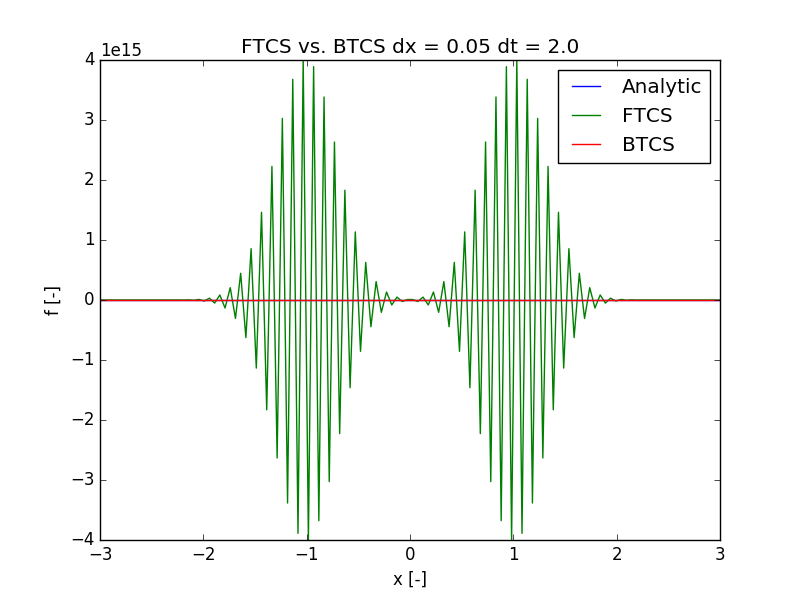
\includegraphics[height=3.75in]{problem2b.png}
	\label{fig:problem2b}
\end{figure}

It is clear from this result that the FTCS scheme is unstable for a time step of 2. This is because the value of $\alpha$ is greater than 0.5 for $\Delta t$ = 2.


%%%%%%%%%%%%%%%%%%%%%%%%%%%%%%%%%%%%%%%%%%%%%%%%%%%%%%%%%%%%%%%%%%%%%%%%%%%%%%%%
% Problem 3

\section{Problem 3}
\noindent
Derive the amplitude ratio G for the Crank-Nicolson scheme.

\begin{equation}
G = \frac{1 - \alpha(1-cos(\theta))}{1 + \alpha(1-cos(\theta))}
\label{eqn:G_og}
\end{equation}
\noindent
The Crank-Nicolson Scheme is as follows:

\begin{equation}
	\frac{f_i^{n+1} - f_i^n}{\Delta t} + O(\Delta T^2) = \frac{K}{2} \left(\frac{f_{i-1}^{n+1} - 2f_i^{n+1} + f_{i+1}^{n+1}}{\Delta x^2} + \frac{f_{i-1}^n - 2f_i^n + f_{i+1}^n}{\Delta x^2}\right) + O(\Delta x^2) 
	\label{eqn:cn_scheme}
\end{equation}

\begin{equation}
f_i^n = A^n exp\left[Ii\theta\right]
\label{eqn:exp_fn}
\end{equation}
	
\begin{equation}
\theta = \frac{2\pi \Delta x}{L}
\end{equation}
\noindent
Equation \ref{eqn:cn_scheme} can be rearranged:

\begin{equation}
 -\alpha f_{i-1}^{n+1} + 2(1-\alpha)f_i^{n+1} -\alpha f_{i+1}^{n+1} = - \alpha f_{i+1}^n + 2(1-\alpha)f_i^n + \alpha f^n_{i+1}
 \label{eqn:cn_unrolled}
\end{equation}
\noindent
Where:

\begin{equation}
	\alpha = \frac{K \Delta t}{\Delta x^2}
\end{equation}
\noindent
Next, a substitution of Equation \ref{eqn:exp_fn} for the f terms in Equation \ref{eqn:cn_unrolled} is performed:
\begin{equation}
\begin{aligned}
	 -\alpha A^{n+1} exp\left[I(i-1)\theta\right] + 2(1-\alpha)A^{n+1} exp\left[I(i)\theta\right] -\alpha A^{n+1} exp\left[I(i+1)\theta\right]\\=\alpha A^{n} exp\left[I(i)\theta\right] + 2(1-\alpha)A^{n} exp\left[I(i)\theta\right] + \alpha A^{n} exp\left[I(i+1)\theta\right]
\end{aligned}
	 \label{eqn:exp_sub}
\end{equation}
\noindent
Now dividing Equation \ref{eqn:exp_sub} by the RHS of Equation \ref{eqn:exp_fn} yields:

\begin{equation}
	-\alpha \frac{A^{n+1}}{A^n} e^{-I\theta} + 2(1+\alpha)\frac{A^{n+1}}{A^n} - \alpha \frac{A^{n+1}}{A^n} e^{I\theta} = \alpha e^{-I\theta} + 2(1-\alpha) + \alpha e^{I\theta}
	\label{eqn:divide_an_term}
\end{equation}
\noindent
From lecture notes we know that, by definition, $\frac{A^{n+1}}{A^n} = G$:

\begin{equation}
-\alpha G e^{-I\theta} + 2(1+\alpha)G - \alpha G e^{I\theta} = \alpha e^{-I\theta} + 2(1-\alpha) + \alpha e^{I\theta}
\label{eqn:sub_G}
\end{equation}
\noindent
From special trig relationships with exponential functions, we get:
\begin{equation}
-2\alpha G cos(\theta) + 2(1+\alpha)G = 2\alpha cos(\theta) + 2(1-\alpha)
\label{eqn:cos_relation}
\end{equation}
\noindent
Solving for G, the relationship is:

\begin{equation}
G = \frac{1 - \alpha(1-cos(\theta))}{1 + \alpha(1-cos(\theta))}
\end{equation}
\noindent
Which of course matches Equation \ref{eqn:G_og}! This value of G is never greater than 1, which means the Crank-Nicolson method is unconditionally stable.
%%%%%%%%%%%%%%%%%%%%%%%%%%%%%%%%%%%%%%%%%%%%%%%%%%%%%%%%%%%%%%%%%%%%%%%%%%%%%%%%

\end{document}